% !TEX encoding = UTF-8 Unicode
% !TEX spellcheck = en-US
% !BIB program = bibtex
%%%%%%%%%%%%%%%%%%%%%%%%%%%%%%%%%%%%%%%%%%%%%%%%%%%%%%%%%%%%%%
%% TEMPLATE DI TESI  
%%!!!!!!!!!!!!!!!!!!!!!ATTENZIONE!!!!!!!!!!!!!!
%% non cancellare nulla fino al commento !!!!FINE!!!! più sotto.
%%
%% © Pietro OLIVA 2022
%%%%%%%%%%%%%%%%%%%%%%%%%%%%%%%%%%%%%%%%%%%%%%%%%%%%%%%%%%%%%%
\UseRawInputEncoding
\documentclass[a4paper, 11pt, oneside]{book}
\usepackage[T1]{fontenc}    % cassetta dei font
\usepackage[utf8]{inputenc} % input encoding 
\usepackage[italian]{babel} % language(s) last one is the main one
\usepackage[margin=3cm, bindingoffset=1cm]{geometry}
\usepackage{listings}
\usepackage{amsfonts,amssymb,amsmath,amsthm,marvosym,wasysym,cancel,physics,bm, mathdots}%tutti simboli matematici possibili


\linespread{1.6}
\usepackage[backend=biber, sorting=none]{biblatex}
\addbibresource{bib.bib}

\usepackage{float}
\usepackage{csquotes}
\usepackage{subfig}

\usepackage{graphicx}
\graphicspath{{./Figure/}}


\usepackage{indentfirst}
\usepackage{fancyhdr}
\setlength{\parindent}{1cm}

\pagestyle{fancy}
\renewcommand{\chaptermark}[1]{\markboth{\thechapter.\ \uppercase{#1}}{}}
\fancyhf{}
\fancyhead[C]{\textbf{\leftmark}}
\fancyfoot[C]{\thepage}
\renewcommand{\headrulewidth}{1pt}
\renewcommand{\footrulewidth}{1pt}
%%%%
%%%% SCEGLI QUALE TI PIACE
%%%%
%\usepackage[Conny]{fncychap}
%\usepackage[Sonny]{fncychap}
%\usepackage[Lenny]{fncychap}
%\usepackage[Glenn]{fncychap}
%\usepackage[Rejne]{fncychap}
%\usepackage[Bjarne]{fncychap}
\usepackage[Bjornstrup]{fncychap}





%%%%%%%%%%%%%%%%%%%%%%%%%%%%%%%%%%%%%%%%%%%%%%%%%%%%%%%%%%%%%%
%% !!!!FINE!!!! più sotto.
%%%%%%%%%%%%%%%%%%%%%%%%%%%%%%%%%%%%%%%%%%%%%%%%%%%%%%%%%%%%%%



%%%%
%%%COSE MOLTO UTILI (ma commentabili)
%%%%
\newcommand{\degree}{\ensuremath{^\circ}}%per il simbolo di gradi
\newcommand{\txtu}[1]{\textsuperscript{#1}}%apice nel testo
\newcommand{\txtd}[1]{\textsubscript{#1}}%pedice nel testo
\newcommand{\bit}{\begin{itemize}}%inizia ambiente item.
\newcommand{\eit}{\end{itemize}}%finisce ambiente item.
\newcommand{\ben}{\begin{enumerate}}%inizia ambiente enumerate.
\newcommand{\een}{\end{enumerate}}%finisce ambiente enumerate.
%\newcommand{\pfrac}[1, 7]{\ensuremath{\frac{\partial #1}{\partial #2}}}%derivata parziale.
\newcommand{\ihat}{\boldsymbol{\hat{\mathbf{\text{\i}}}}}%%VERSORI ijk come dio comanda
\newcommand{\jhat}{\boldsymbol{\hat{\mathbf{\text{\j}}}}}
\newcommand{\khat}{\boldsymbol{\hat{\mathbf{k}}}}


%%%%%%%%%%%%%%%ATTENZIONE!!!
%%% CAPOLETTERA se non piace cancellare
%%% tutto il blocco e togli le iniziali nel corpo
%%%%%%%%%%%%%%%
\usepackage{moresize,anyfontsize}%dimensioni extra
\usepackage{multicol, setspace}%
\usepackage{Acorn, AnnSton, ArtNouv, ArtNouvc, Carrickc, Eichenla, Eileen, EileenBl, Elzevier, GotIn, GoudyIn, Kinigcap, Konanur, Kramer, MorrisIn, Nouveaud, Romantik, Rothdn, Sanremo, Starburst, Typocaps, Zallman}%inserire uno di questi nomi qui: \usefont{U}{   }{xl}{n}  (es. \usefont{U}{ArtNouvc}{xl}{n})
\usepackage[dvipsnames]{xcolor}
\usepackage{lettrine}
\usepackage{yfonts}
\DeclareFontShape{LYG}{ygoth}{m}{n}{ <-> ygoth}{}  %\gothfamily
\DeclareFontShape{LY}{yfrak}{m}{n}{<->yfrak}{}   %\frakfamily
\DeclareFontShape{LY}{yswab}{m}{n}{<->yswab}{}  %\swabfamily
%%%% GIOCA COI FONT SOTTO: SCOMMENTA UNO NUOVO E COMMENTA IL VECCHIO
%\usepackage{tgbonum}
\usepackage{lmodern}
%\usepackage{tgschola}
%\usepackage{antpolt}
%\usepackage{quattrocento}
%\usepackage[sfdefault]{quattrocento}
%\usepackage[light,math]{kurier}
%\usepackage[default]{mintspirit}
%\usepackage{avant}
%\usepackage[scaled=.92]{helvet}%. Sans serif - Helvetica DEFAULT
%\usepackage[sfdefault,light]{roboto}
%\usepackage[sfdefault,thin]{roboto}
%\usepackage[sfdefault]{roboto}
%\usepackage{drm}%ha dei bug ma alla lunga compila
%\usepackage{gfsartemisia}%ha dei bug ma alla lunga compila
%\usepackage[light,math]{iwona}
%\usepackage{accanthis}
%\usepackage{gentium}
%\usepackage[light]{merriweather}
%\usepackage[black]{merriweather}
%\usepackage{tgchorus}
\usepackage{calligra}
%\usepackage{carolmin}
%cambia i font dei capolettera
\ignorespaces\fontseries{b}\fontshape{sl}
\renewcommand{\LettrineTextFont}{\normalfont}
%\usepackage{microtype}
%%%%%%%%%%%%%%%%
%%%%%%%%%%%%%%%%FINE ZONA DA CANCELLARE SE NON PIACE





\title{Tesi}  %% Metti il titolo
\author{Nome Cognome}  %% Metti il tuo nome
%\date{XXXX}



\newenvironment{dedication}
  {\clearpage           % we want a new page
   \thispagestyle{empty}% no header and footer
   \vspace*{\stretch{1}}% some space at the top 
   \itshape             % the text is in italics
   \raggedleft          % flush to the right margin
  }
  {\par % end the paragraph
   \vspace{\stretch{3}} % space at bottom is three times that at the top
   \clearpage           % finish off the page
  }
  
  
  
%%%%INIZIO
\begin{document}

%Frontespizio
\begin{titlepage}
\begin{figure}[H]
        \centering
        
\includegraphics[width=0.9\textwidth]{unicusano.png}
    \end{figure}
   \begin{center}
        \ {\uppercase{\bf {\Large università degli studi Niccolò Cusano}}}\\[5mm]
        %Dipartimento
    	\uppercase{\normalsize Dipartimento di Ingegneria}\\
    \end{center}
    
    \begin{center}
        %Corso di Laurea
    	\normalsize{Corso di Laurea in Ingegneria}\\[20mm]
    	\large{Tesi di laurea}\\[10mm]
    	%Titolo
        {\Huge{\bf Titolo della tesi}}\\[3mm]
    \end{center}
    
   \vspace{20mm}
    \noindent
    \begin{minipage}[t]{0.47\textwidth}
        %Relatore
    	{\large{Relatore:\par\bf Ch.mo Prof.\par Pietro OLIVA}}
    	\vspace{20mm}\\
    	
    \end{minipage}
    \hfill
    \begin{minipage}[t]{0.4\textwidth}\raggedleft
        %Candidato
    	{\large{Candidato:\par \bf Tizio Caio\par Mat.  IN0900xxxx}}
    \end{minipage}
    
    \vfill  
    %Anno Accademico
    \centering{\large \uppercase{Anno Accademico 202X/202X}}
\end{titlepage}

\begin{dedication}

Una dedica ci farà capire chi è per te importante.

\end{dedication}




%%%%%%%%%%%%%%%%%
%%%%%%%%%%Corpo della Tesi
%%%%%%%%%%%%%%%%%


\tableofcontents

\clearpage
\sloppy
\hyphenpenalty=10000
\exhyphenpenalty=10000


\frenchspacing  %% Disabilita un comportamento standard di LaTeX che fa inserire uno spazio supplementare (a volte sgradevole secondo me) dopo un punto, pun.interrogativo o esclamativo e altro. Scegli tu se tenerlo.



\chapter{Introduzione}\label{ch:intro}

\vspace{10mm}

\rightline{``I, at any rate, am convinced that [God] does not throw dice}
\rightline{[Jedenfalls bin ich überzeugt, daß der nicht würfelt.]''}

\rightline{\textit{Albert Einstein, Letter to Max Born}}     
 \vspace{5mm}
 
\lettrine[lines=2, depth=0, lraise=-0.1, findent=0.3em, nindent=0.3em]{\color{BrickRed}\fontsize{50pt}{72pt}L}{orem ipsum} psum dolor sit amet, consectetur adipiscing elit. Curabitur quis massa velit \cite{10.2307/43707814}. Nulla imperdiet rutrum aliquet. Suspendisse imperdiet consequat lectus sed cursus. Nulla tortor nulla, faucibus id lacus non, ultrices tempor turpis. Praesent turpis lacus, pharetra et tortor sed, sagittis ornare turpis. Etiam sodales commodo tristique. Curabitur quis elementum nibh. Quisque id ligula quis orci aliquam sagittis. Vivamus eu tincidunt urna, at elementum lorem. Maecenas vitae urna suscipit, commodo diam sit amet, fermentum lacus. Aenean ultricies laoreet commodo. Maecenas ut aliquet lorem. Donec pulvinar ex sit amet quam viverra semper. Pellentesque vehicula, libero quis tincidunt eleifend, lacus dui feugiat lectus, vel vestibulum magna mauris eget quam. Fusce eu mi nec augue dignissim egestas. 

\chapter{Capitolo}\label{ch:1}

\lettrine[lines=2, depth=0, lraise=-0.1, findent=0.3em, nindent=0.3em]{\color{BrickRed}\fontsize{50pt}{72pt}L}{orem ipsum} dolor sit amet, consectetur adipiscing elit. Curabitur quis massa velit. Nulla imperdiet rutrum aliquet. Suspendisse imperdiet consequat lectus sed cursus. Nulla tortor nulla, faucibus id lacus non, ultrices tempor turpis. Praesent turpis lacus, pharetra et tortor sed, sagittis ornare turpis. Etiam sodales commodo tristique. Curabitur quis elementum nibh. Quisque id ligula quis orci aliquam sagittis. Vivamus eu tincidunt urna, at elementum lorem.

Maecenas vitae urna suscipit, commodo diam sit amet, fermentum lacus. Aenean ultricies laoreet commodo. Maecenas ut aliquet lorem. Donec pulvinar ex sit amet quam viverra semper. Pellentesque vehicula, libero quis tincidunt eleifend, lacus dui feugiat lectus, vel vestibulum magna mauris eget quam. Fusce eu mi nec augue dignissim egestas \cite{20, 33, dep}.

\section{paragrafo}\label{sec:prova}

Aenean cursus lorem in enim finibus, facilisis mattis arcu congue. Curabitur id tortor pulvinar, hendrerit sapien quis, eleifend justo. Donec vitae viverra purus. Aenean non nulla nunc. Morbi non lorem imperdiet, bibendum risus nec, congue nunc. Nulla a ultrices lorem. Vivamus id massa in ligula semper fermentum. Maecenas sed augue mattis, vehicula odio a, interdum erat. Etiam vel tellus vulputate nisi rutrum consectetur a non ante.

\subsection{sottoparagrafo}\label{subsec:prova}

\begin{figure}
    \centering
    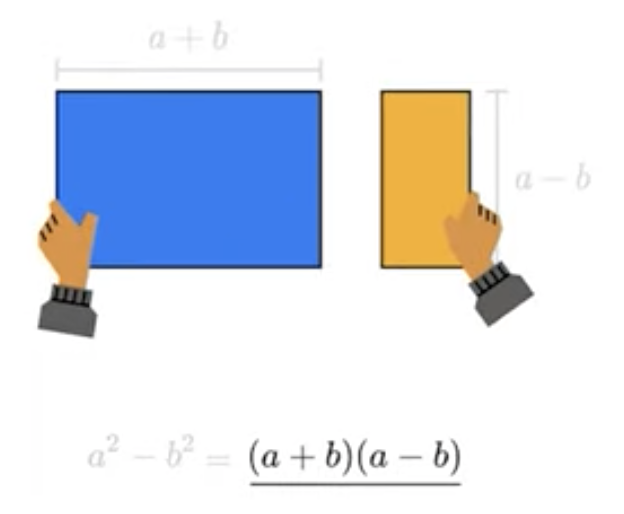
\includegraphics{figura.png}
    \caption{Caption}
    \label{fig:my_label}
\end{figure}

Ut fermentum tempor elit, at pharetra libero dictum facilisis. Maecenas felis nunc, mollis vel auctor eu, ultricies id urna. Donec vel lorem mollis, egestas ipsum at, fringilla massa. Aenean vestibulum odio nibh, in ultrices eros porttitor vitae. Vivamus venenatis, sem et sollicitudin commodo, urna neque cursus elit, vel feugiat lorem elit a nibh. 





\chapter{Capitolo}\label{ch:2}

\lettrine[lines=2, depth=0, lraise=-0.1, findent=0.3em, nindent=0.3em]{\color{BrickRed}\fontsize{50pt}{72pt}L}{orem ipsum} dolor sit amet, consectetur adipiscing elit. Curabitur quis massa velit. Nulla imperdiet rutrum aliquet. Suspendisse imperdiet consequat lectus sed cursus. Nulla tortor nulla, faucibus id lacus non, ultrices tempor turpis. Praesent turpis lacus, pharetra et tortor sed, sagittis ornare turpis. Etiam sodales commodo tristique. Curabitur quis elementum nibh. Quisque id ligula quis orci aliquam sagittis. Vivamus eu tincidunt urna, at elementum lorem. Maecenas vitae urna suscipit, commodo diam sit amet, fermentum lacus. Aenean ultricies laoreet commodo. Maecenas ut aliquet lorem. Donec pulvinar ex sit amet quam viverra semper. Pellentesque vehicula, libero quis tincidunt eleifend, lacus dui feugiat lectus, vel vestibulum magna mauris eget quam. Fusce eu mi nec augue dignissim egestas.

\begin{table}[h!]
    \centering
    \begin{tabular}{c|c}
       Ciao  & Bella \\
       Bella  & Ciao
    \end{tabular}
    \caption{Caption della tabella}
    \label{tab:my_label}
\end{table}
Aenean cursus lorem in enim finibus, facilisis mattis arcu congue. Curabitur id tortor pulvinar, hendrerit sapien quis, eleifend justo. Donec vitae viverra purus. Aenean non nulla nunc. Morbi non lorem imperdiet, bibendum risus nec, congue nunc. Nulla a ultrices lorem. Vivamus id massa in ligula semper fermentum. Maecenas sed augue mattis, vehicula odio a, interdum erat. Etiam vel tellus vulputate nisi rutrum consectetur a non ante. Ut fermentum tempor elit, at pharetra libero dictum facilisis. Maecenas felis nunc, mollis vel auctor eu, ultricies id urna. Donec vel lorem mollis, egestas ipsum at, fringilla massa. Aenean vestibulum odio nibh, in ultrices eros porttitor vitae. Vivamus venenatis, sem et sollicitudin commodo, urna neque cursus elit, vel feugiat lorem elit a nibh. Come si vede in tabella \ref{tab:my_label}.

\chapter{Conclusioni}

\chapter{Ringraziamenti}



\printbibliography


\end{document}
